\documentclass[letterpaper, 11pt]{article}
\usepackage[utf8]{inputenc}
\usepackage[letterpaper, portrait, margin=1in]{geometry}
\usepackage{pgfplots}
\pgfplotsset{width=10cm,compat=1.9}
\usepackage{hyperref}
\usepackage{textcomp}
\usepackage{siunitx}
\usepackage{amsmath}
\usepackage{cancel}
\usepackage{tikz}
\usepackage{everysel}
\usepackage{ragged2e}
\usepackage{mathdots}
\usepackage{yhmath}
\usepackage{color}
\usepackage{array}
\usepackage{multirow}
\usepackage{amssymb}
\usepackage{gensymb}
\usepackage{tabularx}
\usepackage{booktabs}
\usepackage{listings}
\usepackage{xcolor}
\usepackage{enumitem}
\usetikzlibrary{fadings}
\usetikzlibrary{patterns}
\usetikzlibrary{shadows.blur}
\hypersetup{
    colorlinks=true,
    linkcolor=black,
    filecolor=black,      
    urlcolor=blue,
}

\definecolor{codegreen}{rgb}{0,0.6,0}
\definecolor{codegray}{rgb}{0.5,0.5,0.5}
\definecolor{codepurple}{rgb}{0.58,0,0.82}
\definecolor{backcolour}{rgb}{0.95,0.95,0.92}

\lstdefinestyle{mystyle}{
    backgroundcolor=\color{backcolour},   
    commentstyle=\color{codegreen},
    keywordstyle=\color{magenta},
    numberstyle=\tiny\color{codegray},
    stringstyle=\color{codepurple},
    basicstyle=\ttfamily\footnotesize,
    breakatwhitespace=false,         
    breaklines=true,                 
    captionpos=b,                    
    keepspaces=true,                 
    numbers=left,                    
    numbersep=5pt,                  
    showspaces=false,                
    showstringspaces=false,
    showtabs=false,                  
    tabsize=2
}

\lstset{style=mystyle}

\title{COMSC-200 \\ Lab 10}
\author{Ryan Jacoby}
\date{8 November 2020}
\begin{document}

\maketitle

\section{R14.27}
In our circular array implementation of a queue, can you compute the value of len from the values of the \textit{head} and \textit{tail} data members?  Why or why not? \\

No, the len must be kept track of or can be calculated if the head and tail are kept track of.  There is no way to calculate the length from the values stored at head and tail, but it is easy to calculate len if the locations of head and tail are known along with the capacity of the circular array.

\section{E14.21}
I currently do not have access to the textbook; I will e-mail you my solution when I do.

\section{Infix to Postfix Conversion}

\begin{lstlisting}[language=c++, caption=main.cpp]
// Ryan Jacoby

#include<iostream>
#include<stack>
#include<string>

using namespace std;

string convertToPostfix(stack<char>);

int main() {
    stack<char> equation;

    equation.push('x');
    equation.push('+');
    equation.push('y');
    equation.push('*');
    equation.push('z');

    cout << "x+y*z converted to postfix is: ";
    cout << convertToPostfix(equation) << '\n';

    return 0;
}

string convertToPostfix(stack<char> infix) {
    stack<char> operatorStack = stack<char>();
    string postfix = "";

    while(!infix.empty()) {
        char nextCharacter = infix.top();
        infix.pop();
        switch(nextCharacter) {
            case 'a' : case 'b' : case 'x' : case 'y' : case 'z':
                postfix += nextCharacter;
                break;
            case '^':
                operatorStack.push(nextCharacter);
                break;
            case '+' : case '-' : case '*' : case '/':
                while(!operatorStack.empty()) { // Implement elegant way of anding with operator precedence; nextChar <= operatorStack.top();
                    postfix += operatorStack.top();
                    operatorStack.pop();
                }
                operatorStack.push(nextCharacter);
                break;
            case '(':
                operatorStack.push(nextCharacter);
                break;
            case ')':
                {
                    char topOperator = operatorStack.top();
                    operatorStack.pop();
                    while(topOperator != '(') {
                        postfix += topOperator;
                        topOperator = operatorStack.top();
                        operatorStack.pop();
                    }
                    break;
                }
            default: break;
        }
    }

    char topOperator;
    while(!operatorStack.empty()) {
        topOperator = operatorStack.top();
        operatorStack.pop();
        postfix += topOperator;
    }

    return postfix;
}
\end{lstlisting}

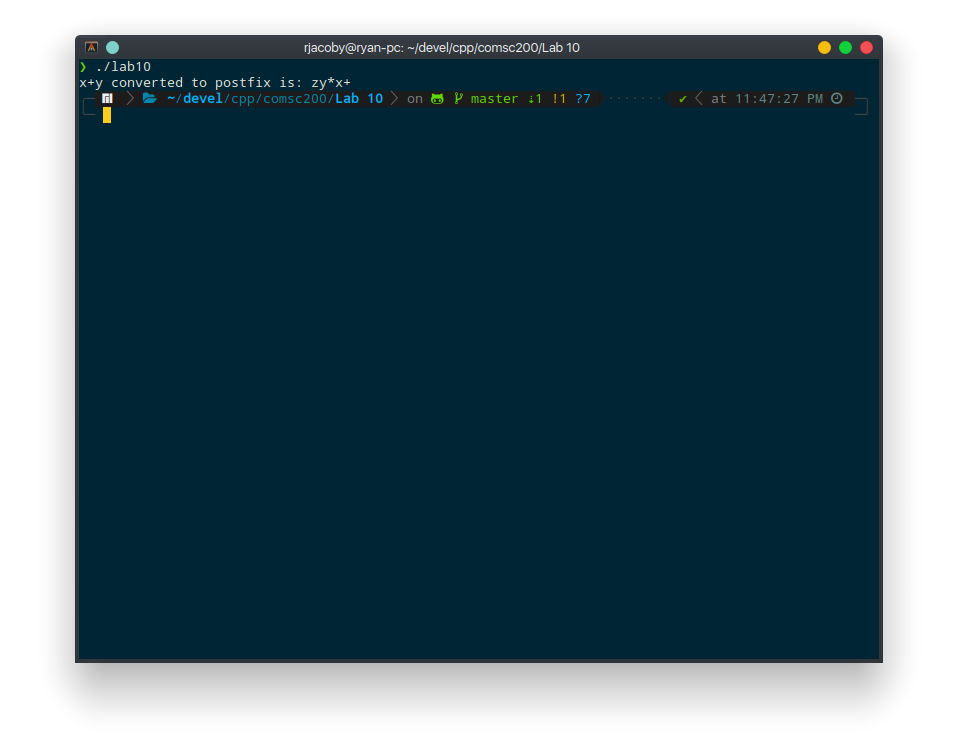
\includegraphics[scale=0.5]{infix_postfix.png}

\end{document}
